\documentclass[czech]{pyt-report}

\usepackage[utf8]{inputenc} 

\title{Boulder Dash 1984 Remake}

\author{Lukáš Bien}
\affiliation{ČVUT--FIT}
\email{bienluka@fit.cvut.cz}

\def\file#1{{\tt#1}}

\begin{document}

\maketitle

%%%%%%%%%%%%%%%%%%%%%%%%%%%%%%%%%%%%%%%%%%%%%%%%%%%%%%%%%%%%%%%%%%%%%%%%%%%%%%%%
\section{Úvod}

\subsection{Cíle}
Cílem semestrální práce bylo vytvořit hratelný remake hry \emph{Boulder Dash} (1984) v jazyce Python s využitím knihovny \texttt{pyglet} \cite{pyglet}.
Projekt je implementován jako dlaždicová hra s tick systémem --- fyzika a chování objektů se vyhodnocuje periodicky.

Hlavní cíle projektu:
\begin{itemize}
  \item implementovat machaniky hry --- pohyb hráče, posouvání kamenů, sbírání drahokamů, pohyb nepřátel\ldots
  \item implementovat gravitaci pro kameny a drahokamy
  \item uživatelské rozhraní --- zobrazení skóre, počet nasbíraných drahokamů, zbývající čas\ldots
  \item načítání úrovní (levelů) z textových souborů
\end{itemize}

Projekt je určen pro vzdělávací, nekomerční použití. Použité zdroje grafiky, fontu a dat úrovní jsou uvedeny v souboru \file{assets/CREDITS.txt}.

%%%%%%%%%%%%%%%%%%%%%%%%%%%%%%%%%%%%%%%%%%%%%%%%%%%%%%%%%%%%%%%%%%%%%%%%%%%%%%%%
\section{Vstupní data}

\subsection{Formát úrovní}
Úrovně jsou uloženy ve formátu TOML v adresáři \file{assets/levels/}. Každý soubor obsahuje meta informace (např. název, časový limit, počet požadovaných drahokamů) a ASCII mapu dlaždic. Při načtení se jednotlivé znaky mapují na interně definované typy dlaždic.

\begin{figure}[h]
    \centering\leavevmode
    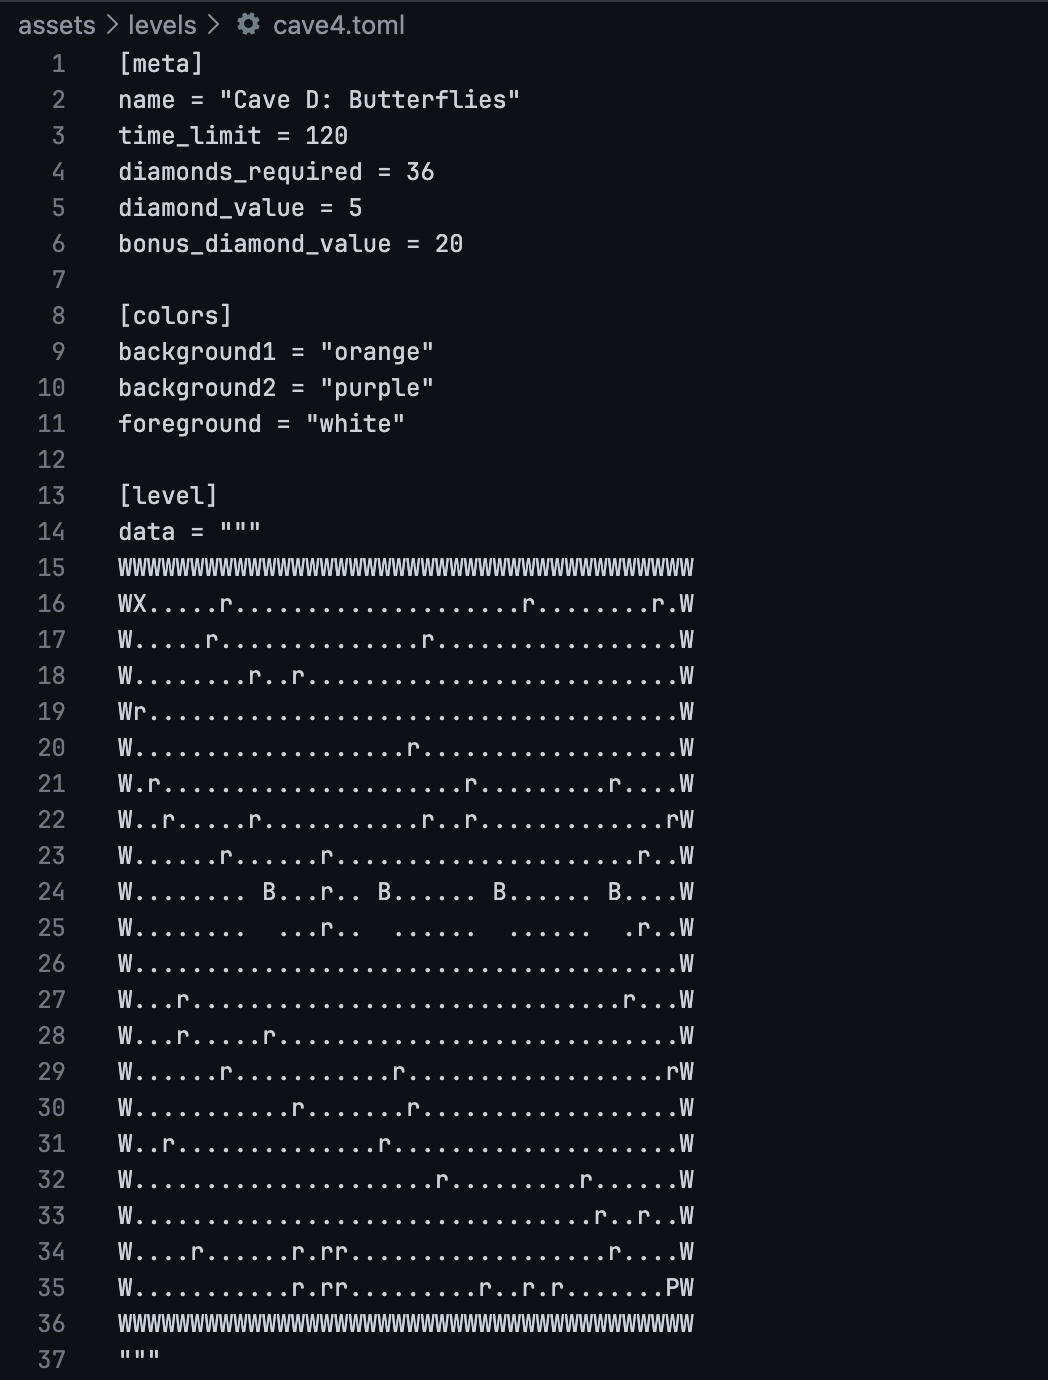
\includegraphics[width=0.85\linewidth]{img/level.png}
    \caption{Příklad TOML souboru popisující jednu úroveň.}
    \label{fig:level}
\end{figure}

Konfigurace hry je uložena v YAML souboru \file{game/cfg/config.yaml} a načítá se pomocí knihovny PyYAML \cite{pyyaml}.

\subsection{Původ dat}
Základní rozložení urovní vychází z dekódovaných dat původní verze (C64) publikovaných Jake Gordonem \cite{caves}. Grafický spritesheet je převzat ze stejného zdroje a byl barevně upraven \cite{sprites}. Použitý font \uv{Boulder Dash 6128} pochází z portálu dafont \cite{font}.

%%%%%%%%%%%%%%%%%%%%%%%%%%%%%%%%%%%%%%%%%%%%%%%%%%%%%%%%%%%%%%%%%%%%%%%%%%%%%%%%
\section{Metody/postupy/algoritmy}
\subsection{Architektura}
Aplikace je rozdělena na několik hlavních částí:
\begin{itemize}
    \item \file{game/game.py}: řízení stavu hry (skóre, životy, čas, přechod úrovní), zpracování vstupu.
    \item \file{game/lvl/level.py}: načítání úrovní a herní simulace (fyzika, nepřátele\ldots).
    \item \file{game/gfx/renderer.py}: vykreslování dlaždic a uživatelského rozhraní.
    \item \file{game/cfg/config.py}: načítání konfigurace.
\end{itemize}

\subsection{Simulace herní fyziky}
Fyzika kamenů a drahokamů je vyhodnocována po částech. Pro každou aktualizace se nejprve vytvoří kopie typů dlaždic a stavů \uv{falling} a poté se aplikuje sada pravidel:
\begin{itemize}
    \item volný pád do prázdné buňky,
    \item rozdělení \uv{falling} vs. \uv {stojící} objekt (např. zabití hráče jen při dopadu padajícího objektu),
    \item sklouzávání z kulatých povrchů (pravidla pro \uv{rounded} dlaždice),
    \item zabití nepřátel padajícím objektem (butterfly vytvoří shluk drahokamů).
\end{itemize}

\subsection{Nepřátele}
V projektu jsou implementovány dva typy nepřátel: \emph{firefly} a \emph{butterfly}. Oba se pohybují po mřížce podle pravidla \uv{následování stěny} (wall following). Kontakt s hráčem vede k jeho smrti.

Butterfly má specifické chování při smrti: vytvoří ve svém okolí $3\times3$ drahokamy.

\subsection{Amoeba}
Amoeba se náhodně rozrůstá do sousedních prázdných nebo \uv{dirt} buněk s určitou pravděpodobností. Pokud se amoeba \uv{uzavře} (nemá kam růst), transformuje se na drahokamy. Pokud překoná maximální velikost, transformuje se na kameny.

\subsection{Magic wall}
Magic wall (magická stěna) transformuje padající objekty: kámen \textrightarrow{} diamant a diamant \textrightarrow{} kámen. Transformace probíhá jen v případě, že je výstupní buňka pod stěnou volná.

\begin{figure}[h]
    \centering\leavevmode
    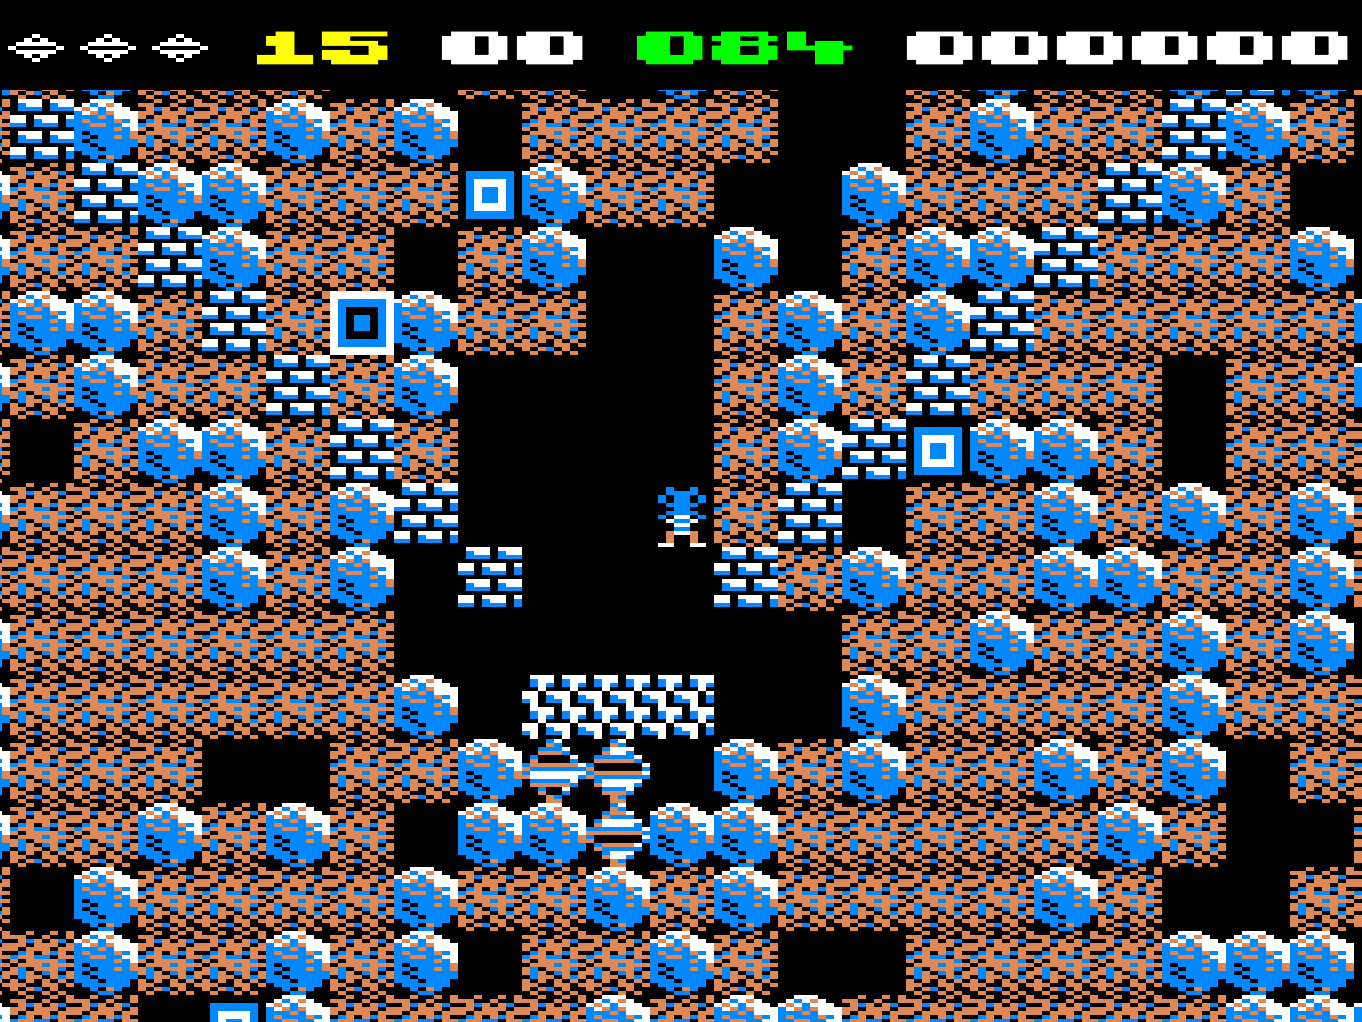
\includegraphics[width=0.85\linewidth]{img/magicwall.png}
    \caption{Magic wall (třetí buňka pod hráčem).}
    \label{fig:magicwall}
\end{figure}

\subsection{Testování}
Projekt obsahuje jednotkové testy spustitelné příkazem \texttt{pytest} \cite{pytest}. Pro testy je hra schopna běžet v \uv{headless} režimu bez vytvoření okna, aby testy běžely rychle.

%%%%%%%%%%%%%%%%%%%%%%%%%%%%%%%%%%%%%%%%%%%%%%%%%%%%%%%%%%%%%%%%%%%%%%%%%%%%%%%%
\section{Výsledky}

Výsledkem je funkční hra s 20 úrovněmi, základním uživatelským rozhraním a implementovanými mechanikami popsanými v předchozích sekcích. Při prohře se zobrazí \uv{game over} s finálním získaným počtem skóre a hru lze restartovat podržením klávesy \uv{R}.


\begin{figure}[h]
    \centering\leavevmode
    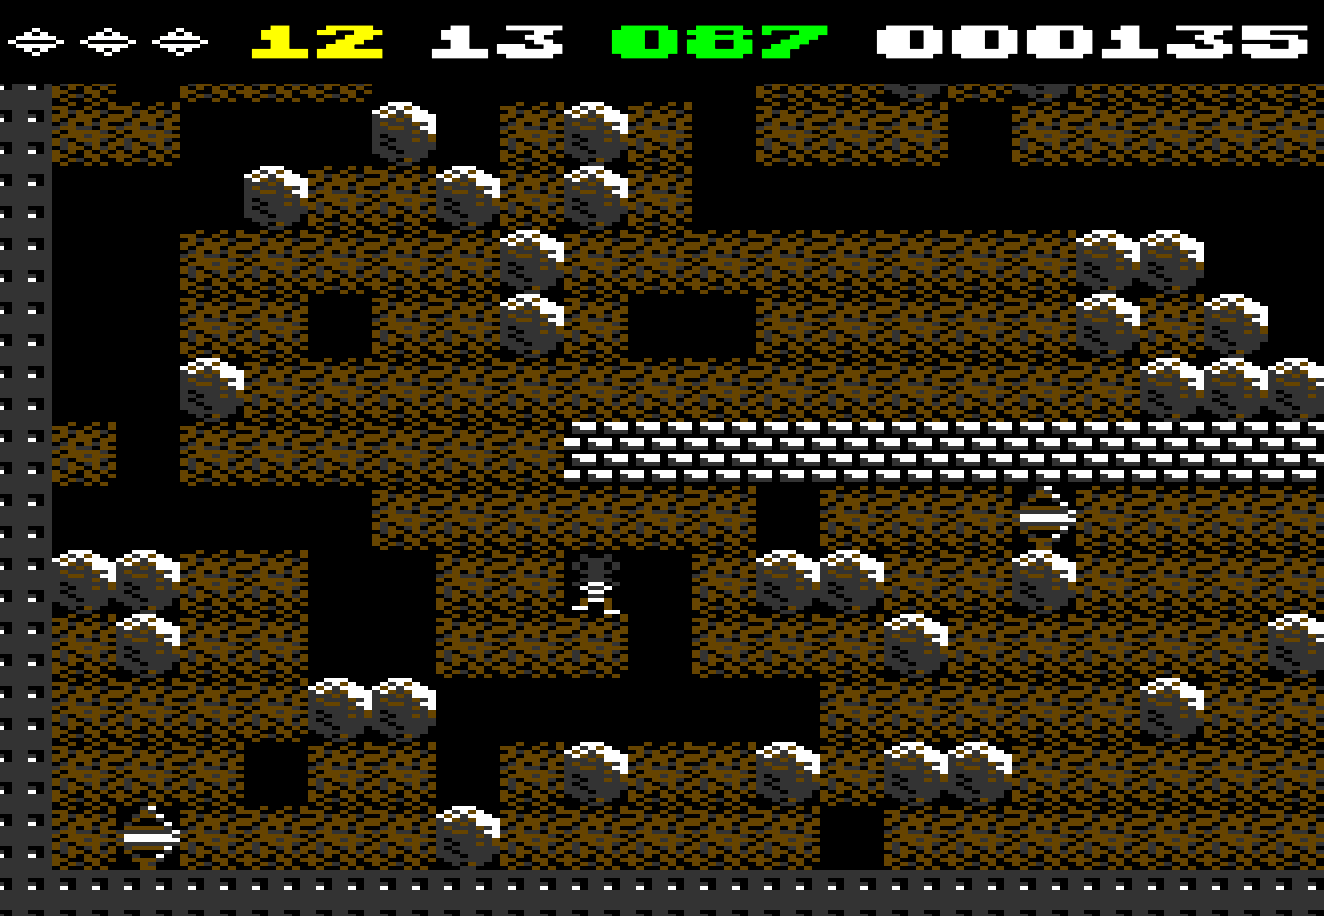
\includegraphics[width=.85\linewidth]{img/game.png}
    \caption{Ukázka hry.}
    \label{fig:game}
\end{figure}
\begin{figure}[h]
    \centering\leavevmode
    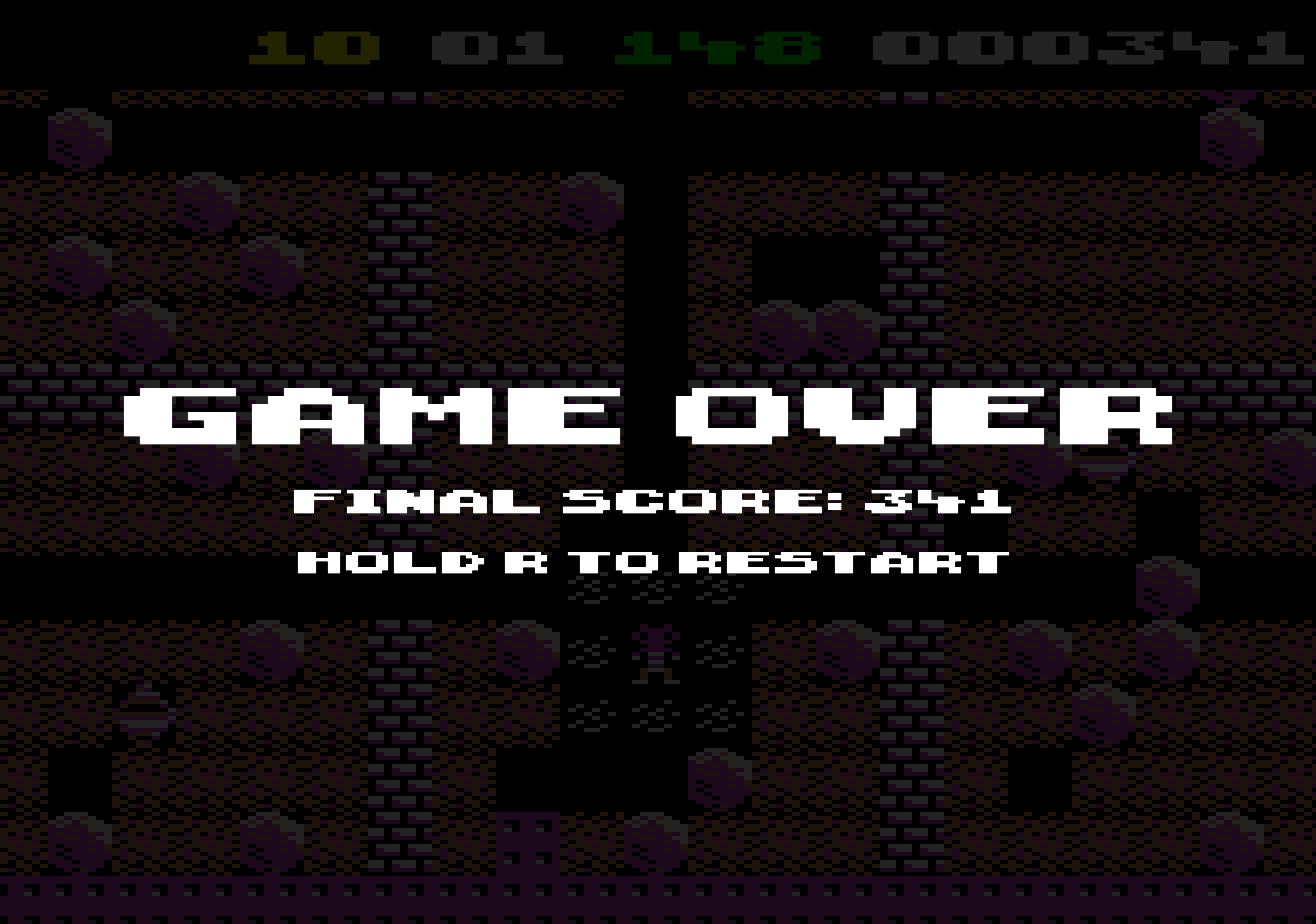
\includegraphics[width=0.85\linewidth]{img/gameover.png}
    \caption{Konec hry s finálním skóre.}
    \label{fig:gameover}
\end{figure}

%%%%%%%%%%%%%%%%%%%%%%%%%%%%%%%%%%%%%%%%%%%%%%%%%%%%%%%%%%%%%%%%%%%%%%%%%%%%%%%%
\section{Závěr}
Projekt naplnil cíl vytvořit remake hry Boulder Dash s klíčovými herními mechanikami.
Mezi možná budoucí vylepšení patří zlepšení pravidel tak, aby více odpovídala originálu, vylepšení uživatelského rozhraní, či opravení různých vizuálních chyb. Projekt také může sloužit jako jednoduchá ukázka jak použít knihovnu \texttt{pyglet} \cite{pyglet}. 

%%%%%%%%%%%%%%%%%%%%%%%%%%%%%%%%%%%%%%%%%%%%%%%%%%%%%%%%%%%%%%%%%%%%%%%%%%%%%%%%
% --- Bibliography
\nocite{sprites}
\nocite{caves}
\nocite{font}
\nocite{pyglet}
\nocite{pytest}
\nocite{pyyaml}
%\bibliographystyle{plain-cz-online}
\bibliography{reference}

\end{document}
